% Assignment1 - Ajeesh T. Vijayan
\documentclass[11pt,a4paper]{article}
\usepackage[utf8]{inputenc}
\usepackage{array}
\usepackage{caption}
\usepackage{enumerate}
\usepackage{amsmath, amssymb}
\usepackage{array, makecell}
\usepackage{booktabs}
\usepackage{graphicx}
\usepackage[left=2.5cm,right=1.5cm,top=2cm,bottom=1.5cm]{geometry}
\usepackage{wrapfig}
\usepackage{float}
\usepackage{fancyhdr}
\usepackage[colorlinks=true]{hyperref}
\usepackage{listings, lstautogobble}
\usepackage{listings-rust}
\usepackage{xcolor}
\usepackage{fontawesome5}
\usepackage{adjustbox}


%New colors defined below
\definecolor{codegreen}{rgb}{0,0.6,0}
\definecolor{codegray}{rgb}{0.5,0.5,0.5}
\definecolor{codepurple}{rgb}{0.58,0,0.82}
\definecolor{backcolour}{rgb}{0.95,0.95,0.92}

%Code listing style named "mystyle"
\lstdefinestyle{mystyle}{
	backgroundcolor=\color{backcolour},   commentstyle=\color{codegreen},
	keywordstyle=\color{magenta},
	numberstyle=\tiny\color{codegray},
	stringstyle=\color{codepurple},
	basicstyle=\ttfamily\footnotesize,
	breakatwhitespace=false,         
	breaklines=true,                 
	captionpos=b,                    
	keepspaces=true,                 
	numbers=left,                    
	numbersep=3pt,                  
	showspaces=false,                
	showstringspaces=false,
	showtabs=false,                  
	tabsize=2
}

%"mystyle" code listing set
\lstset{style=mystyle}

\lstdefinestyle{DOS}
{
	backgroundcolor=\color{black},
	basicstyle=\scriptsize\color{white}\ttfamily
}

\def\ie{\latinabbrev{i.e}}

\makeatletter
\newcommand{\github}[1]{%
	\href{#1}{\faGithubSquare}%
}
\makeatother

\captionsetup[table]{position=bottom}   %% or below

\pagestyle{fancy}
\lhead{Ajeesh T. Vijayan}
\rhead{Student No: 22077273}
\cfoot{\thepage}
\renewcommand{\headrulewidth}{0.4pt}
\renewcommand{\footrulewidth}{0.4pt}

\title{MA7010 – Number Theory for Cryptography - Assignment 1}
\author{Ajeesh Thattukunnel Vijayan}
\date{January 11\textsuperscript{th} 2024}

\newenvironment{numberlists}[1][3\parindent]
{\begin{list}{}{%
			\leftmargin=#1\relax
			\rightmargin=\leftmargin
			\itemsep=\jot
			\parsep=0pt
			\partopsep=0pt
			\labelsep=0pt}}
	{\end{list}}

\newcommand\numlist[2]{%
	\item[]\makebox[0pt][r]{$#1=\lbrack$}%
	\begingroup
	\begingroup\lccode`~=`,\lowercase{\endgroup\def~}{\mathcomma\penalty0 }%
	\mathcode`,="8000
	\thinmuskip=6mu plus 6mu minus 2mu
	$#2\rbrack$%
	\endgroup
}

\definecolor{dkgreen}{rgb}{0,0.6,0}
\definecolor{gray}{rgb}{0.5,0.5,0.5}
\definecolor{mauve}{rgb}{0.58,0,0.82}

\mathchardef\mathcomma=\mathcode`,
\newcommand{\roverline}[1]{\mathpalette\doroverline{#1}}
\newcommand{\doroverline}[2]{\overline{#1#2}}

\begin{document}
	
	\maketitle
	\section{Notes} \label{sec:Intro}
 	I have used a combination of Maple and Rust Code to arrive at the solutions. The code snippets presented in this document are in Rust. I developed the code using the u64 primitive datatype in Rust and later changed that to \href{https://docs.rs/num-bigint/0.4.4/num_bigint/}{BigInt} with the hope that I could use very large Integers such as more than 500bits long, but it became a challenge. Many times computer terminated the execution with Out Of Memory errors.
	\section{Answers} \label{sec:Forces}
	
	\begin{enumerate}[1.]
		\item Lower Range = 2800, Upper Range = 3100.
		\begin{enumerate}[(a)]
			\item List the elements of the set A = {all primes p in the range}, B = {all composite numbers in the range}.
		\end{enumerate}
		\begin{flushleft}
			\textbf{\textit{Answer:}}
			\begin{numberlists}
				\numlist{Primes}{2801, 2803, 2819, 2833, 2837, 2843, 2851, 2857, 2861, 2879, 2887, 2897, 2903, 2909, 2917, 2927, 2939, 2953, 2957, 2963, 2969, 2971, 2999, 3001, 3011, 3019, 3023, 3037, 3041, 3049, 3061, 3067, 3079, 3083, 3089}
				
				\numlist{Composites}{2800, 2802, 2804, 2805, 2806, 2807, 2808, 2809, 2810, 2811, 2812, 2813, 2814, 2815, 2816, 2817, 2818, 2820, 2821, 2822, 2823, 2824, 2825, 2826, 2827, 2828, 2829, 2830, 2831, 2832, 2834, 2835, 2836, 2838, 2839, 2840, 2841, 2842, 2844, 2845, 2846, 2847, 2848, 2849, 2850, 2852, 2853, 2854, 2855, 2856, 2858, 2859, 2860, 2862, 2863, 2864, 2865, 2866, 2867, 2868, 2869, 2870, 2871, 2872, 2873, 2874, 2875, 2876, 2877, 2878, 2880, 2881, 2882, 2883, 2884, 2885, 2886, 2888, 2889, 2890, 2891, 2892, 2893, 2894, 2895, 2896, 2898, 2899, 2900, 2901, 2902, 2904, 2905, 2906, 2907, 2908, 2910, 2911, 2912, 2913, 2914, 2915, 2916, 2918, 2919, 2920, 2921, 2922, 2923, 2924, 2925, 2926, 2928, 2929, 2930, 2931, 2932, 2933, 2934, 2935, 2936, 2937, 2938, 2940, 2941, 2942, 2943, 2944, 2945, 2946, 2947, 2948, 2949, 2950, 2951, 2952, 2954, 2955, 2956, 2958, 2959, 2960, 2961, 2962, 2964, 2965, 2966, 2967, 2968, 2970, 2972, 2973, 2974, 2975, 2976, 2977, 2978, 2979, 2980, 2981, 2982, 2983, 2984, 2985, 2986, 2987, 2988, 2989, 2990, 2991, 2992, 2993, 2994, 2995, 2996, 2997, 2998, 3000, 3002, 3003, 3004, 3005, 3006, 3007, 3008, 3009, 3010, 3012, 3013, 3014, 3015, 3016, 3017, 3018, 3020, 3021, 3022, 3024, 3025, 3026, 3027, 3028, 3029, 3030, 3031, 3032, 3033, 3034, 3035, 3036, 3038, 3039, 3040, 3042, 3043, 3044, 3045, 3046, 3047, 3048, 3050, 3051, 3052, 3053, 3054, 3055, 3056, 3057, 3058, 3059, 3060, 3062, 3063, 3064, 3065, 3066, 3068, 3069, 3070, 3071, 3072, 3073, 3074, 3075, 3076, 3077, 3078, 3080, 3081, 3082, 3084, 3085, 3086, 3087, 3088, 3090, 3091, 3092, 3093, 3094, 3095, 3096, 3097, 3098, 3099, 3100}
			\end{numberlists}

			\bigbreak
			\bigbreak
			The below images depicts the execution of the code on a powershell terminal:

			\begin{minipage}{\linewidth}
				\begin{center}
					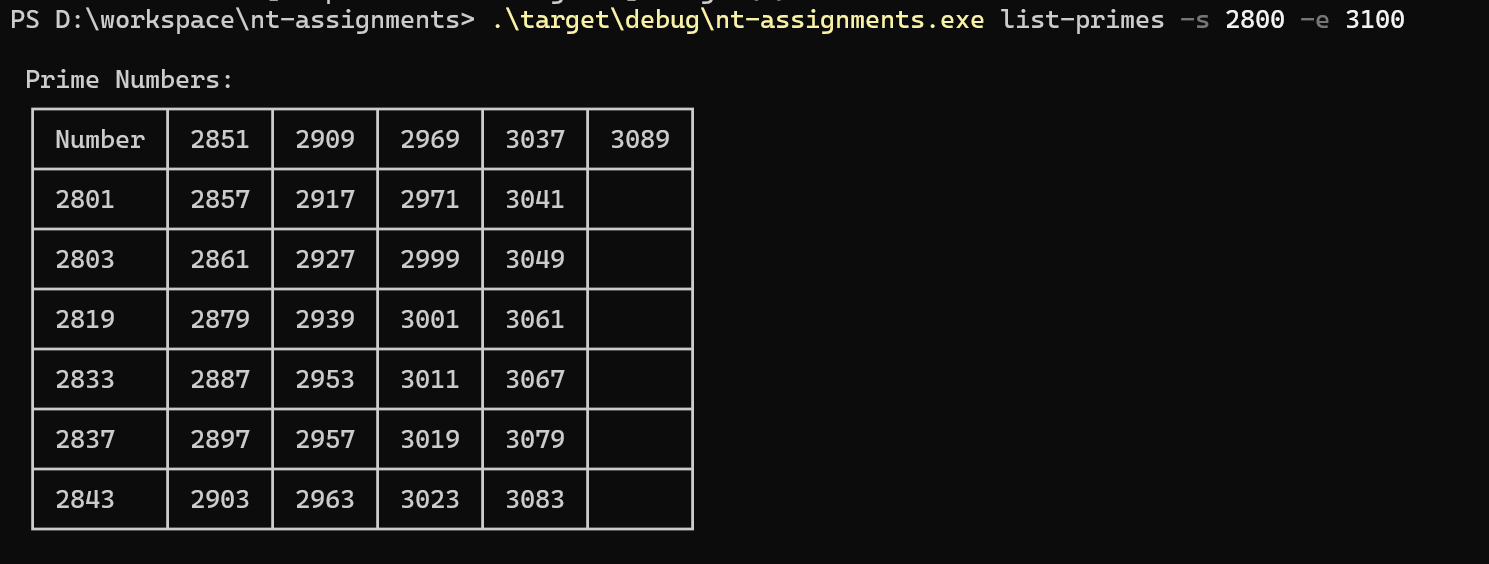
\includegraphics[scale=.45]{primes.png}
					\captionof{figure}{Prime Numbers - Code Execution Output}
					\label{figure1:primes}
				\end{center}
			\end{minipage}
			
			\bigbreak
			\bigbreak
			\begin{minipage}{\linewidth}
				\begin{center}
				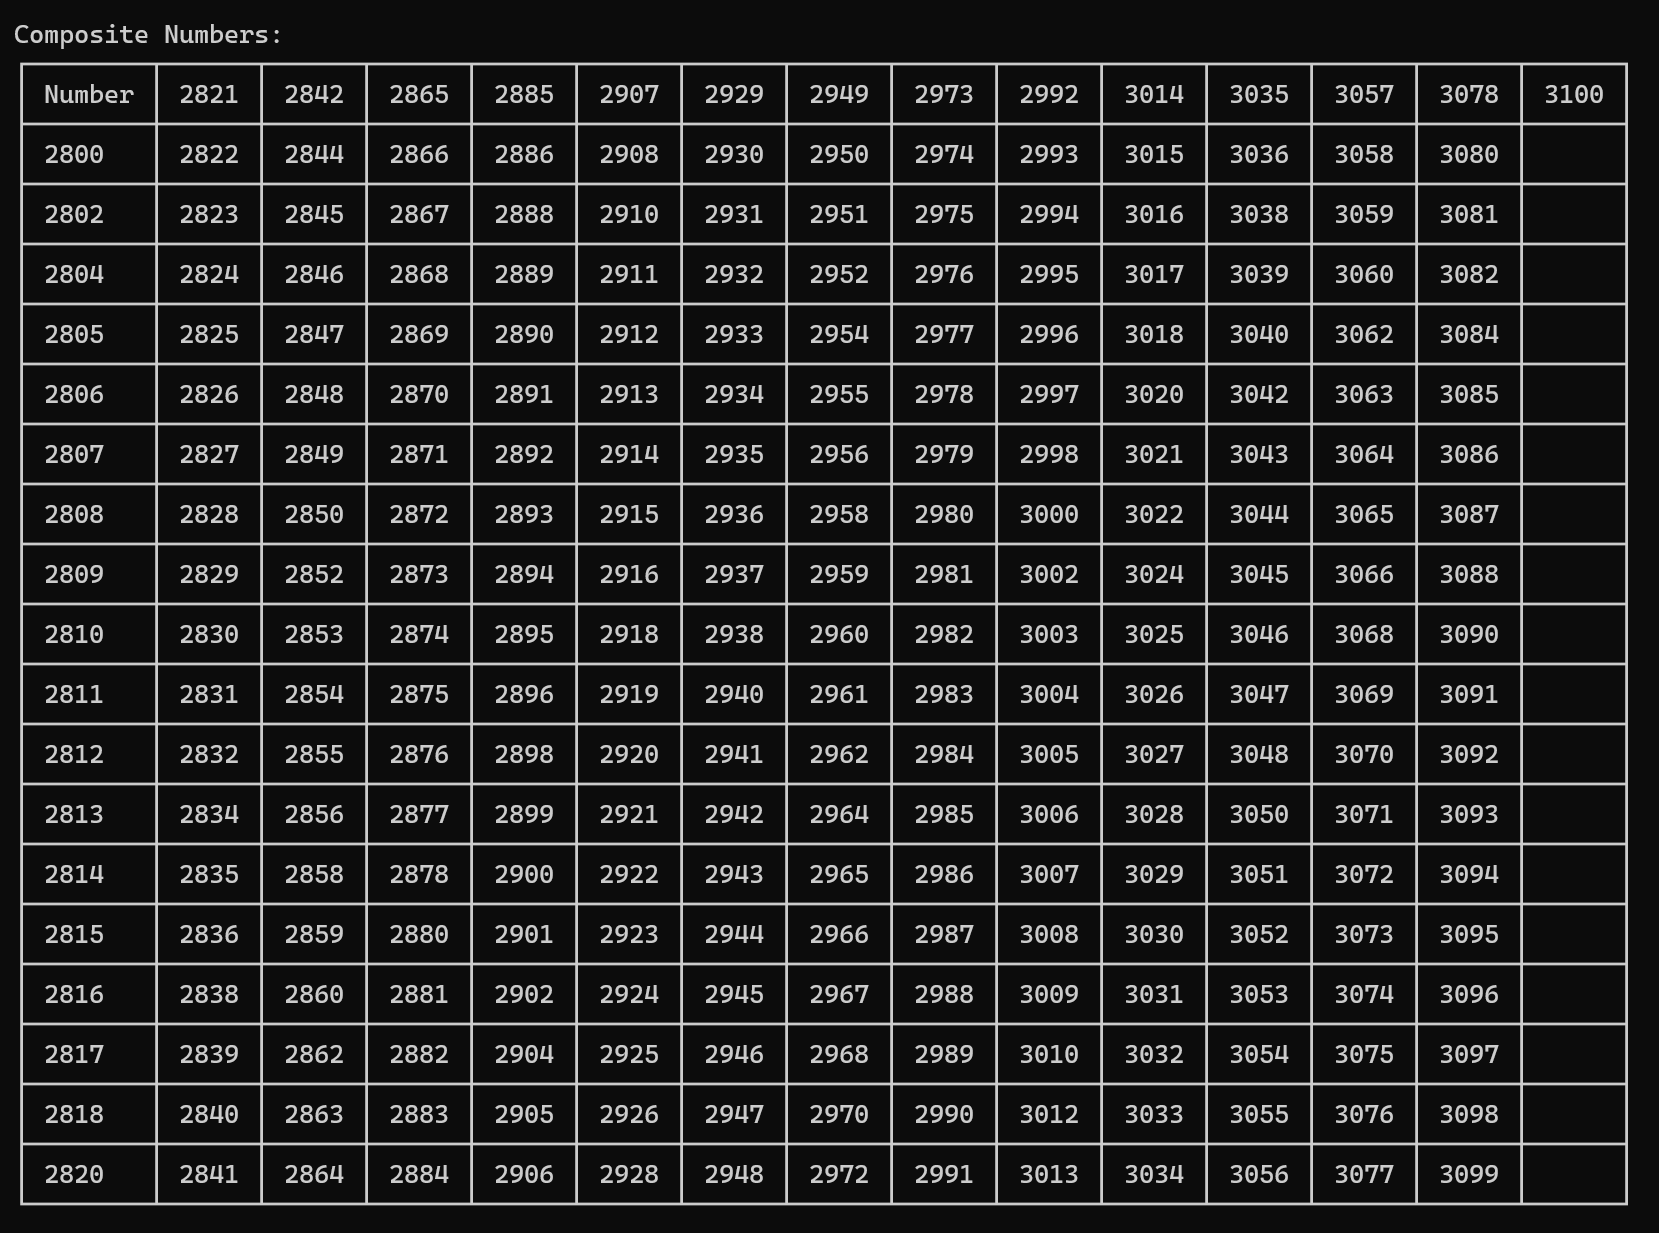
\includegraphics[scale=.45]{composites.png}
				\captionof{figure}{Composite Numbers - Code Execution Output}
				\label{figure2:composites}
				\end{center}
			\end{minipage}
			
			\bigbreak
			\bigbreak
			Code Snippet - Prime Number Sieve
			\begin{lstlisting}[
				language=Rust, 
				basicstyle=\tiny, 
				caption=Prime Number Sieve
				\github{https://github.com/a11e6s8vt/nt-assignments/blob/afec32c31963cb295f7c86719dec6d0792081ee8/src/primality.rs\#L57}        
			]

			/// Returns a boolean representing if the given number is prime or not
			///
			/// # Arguments
			///
			/// * `n` - A BigInt
			///
			/// # Examples
			///
			/// ```
			/// use crate::primality::is_prime_trial_division_parallel;
			/// let is_prime = is_prime_trial_division_parallel(BigInt::from(100u64));
			/// ```
			pub fn is_prime_trial_division_parallel(n: &BigInt) -> bool {
				let (zero, one, _two) = (BigInt::from(0u64), BigInt::from(1u64), BigInt::from(2u64));
				let three = BigInt::from(3u64);
				
				// returns true if the number is 2 or 3
				if n <= &three {
					return n > &one;
				}
				
				if n % 2 == zero || n % 3 == zero {
					return false;
				}
				
				let upper_bound = n.sqrt() + 1; // +1 to get the ceiling value
				
				if let Some(_divisor) = range_inclusive(BigInt::from(5u64), upper_bound)
				.par_bridge()
				.into_par_iter()
				.find_first(|divisor| n % divisor == zero)
				{
					false
				} else {
					true
				}
			}

			
			\end{lstlisting}

			The above code verifies the primality of a number using trial division. It generates a sequence of numbers from $2$ to $sqrt(n) + 1$ and divides these numbers into chunks of blocks and checks the divisibility in parallel to speed up the execution. The parallelisation library used for this purpose is \href{https://crates.io/crates/rayon}{Rayon}
			
			\bigbreak
			The below command execute the Prime Number Sieve:
			\begin{lstlisting}[style=DOS, caption=Example command - Prime Number Sieve]

			.\nt-assignments.exe list-primes -s 2800 -e 3100
			\end{lstlisting}
		\end{flushleft}
		
		\begin{enumerate}[(b)]
			\item List the elements of the set C where C = \{composite numbers n = pq in your range which are the product of exactly two distinct primes p and q\}.
		\end{enumerate}
		\begin{flushleft}
			\textbf{\textit{Answer:}} The code snippet below extracts the numbers of the form $n = p.q$
			\begin{lstlisting}[
				language=Rust, 
				basicstyle=\tiny, 
				caption=Prime Factorisation
				\github{https://github.com/a11e6s8vt/nt-assignments/blob/afec32c31963cb295f7c86719dec6d0792081ee8/src/primality.rs\#L57}        
				]
				
			///
			/// Returns a tuple with a formatted string for output and a Vector which contains a tuple of
			/// Number and its prime factors
			///
			/// # Arguments
			/// * `start` - BigInt
			/// * `end` - BigInt
			/// * `NumCategory` - Whether we want the prime factorisation of All numbers or composites or composits of the form P.Q
			/// # Example
			/// ```
			/// use crate::presets::list_prime_factors_in_range;
			/// list_prime_factors_in_range(&start, &end, NumCategory::All);
			/// ```
			pub fn list_prime_factors_in_range(
			start: &BigInt,
			end: &BigInt,
			opts: NumCategory,
			) -> (Vec<NumFactorTable>, Vec<(BigInt, Vec<(BigInt, usize)>)>) {
				let mut table_data: Vec<NumFactorTable> = Vec::new();
				let mut primes = vec![BigInt::from(2u64)];
				let mut nums_pfactors: Vec<(BigInt, Vec<(BigInt, usize)>)> = Vec::new();
				for num in range_inclusive(start.clone(), end.clone()) {
					let mut form: String = String::new();
					let p_factors = num.prime_factors(&mut primes);
					match opts {
						NumCategory::All => {
							format_prime_factors_print(&num, &p_factors, &mut form, &mut table_data);
							nums_pfactors.push((num.clone(), p_factors.clone()));
						}
						NumCategory::Composites => {
							if p_factors.len() >= 2 {
								format_prime_factors_print(&num, &p_factors, &mut form, &mut table_data);
								nums_pfactors.push((num.clone(), p_factors.clone()));
							}
						}
						NumCategory::CompositesPQ => {
							if p_factors.len() == 2 {
								let first = p_factors.first().unwrap();
								let second = p_factors.get(1).unwrap();
								
								match first.1 {
									1 => match second.1 {
										1 => {
											format_prime_factors_print(
											&num,
											&p_factors,
											&mut form,
											&mut table_data,
											);
											nums_pfactors.push((num.clone(), p_factors.clone()));
										}
										_ => {}
									},
									_ => {}
								}
							}
						}
						NumCategory::Primes => {}
					}
				}
				
				(table_data, nums_pfactors)
			}
				
			pub trait PrimeFactors {
				fn prime_factors(&self, primes: &mut Vec<BigInt>) -> Vec<(BigInt, usize)>;
				//fn is_prime_factors_form_pq(&self) -> (bool, Vec<(BigInt, usize)>);
			}
			
			impl PrimeFactors for BigInt {
				fn prime_factors(&self, primes: &mut Vec<BigInt>) -> Vec<(Self, usize)> {
					let n = self.clone();
					// Check if n is prime
					if miller_rabin_primality(&self) {
						return vec![(self.clone(), 1)];
					}
					
					let start_no = primes.last().unwrap();
					let square_root = self.sqrt();
					if square_root - start_no > BigInt::from(2u64) {
						let end_no: BigInt = self.sqrt() + 1; // +1 to get the ceiling value
						// println!("start = {}, end = {}", start_no, end_no);
						
						let r = range_inclusive(start_no.clone(), end_no);
						
						let new_primes: Vec<BigInt> = r
						.into_iter()
						.map(|x| x)
						.parallel_filter(|x| miller_rabin_primality(x))
						.collect();
						primes.extend(new_primes);
						let mut seen = HashSet::new();
						primes.retain(|c| seen.insert(c.clone()));
					}
					let _res: HashMap<BigInt, usize> = HashMap::new();
					
					// The all_divisors vec will contain all the divisors of num with repetition.
					// The product of the elements of all_divisors will equal the "num"
					let mut all_divisors = Vec::<BigInt>::new(); //
					let mut product = BigInt::one();
					
					while product < n {
						let divisors = primes
						.par_iter()
						.filter(|x| (n.clone() / &product) % *x == BigInt::zero())
						.map(|p| p.clone())
						.collect::<Vec<BigInt>>();
						all_divisors.extend(divisors.clone());
						product = product
						* divisors
						.iter()
						.fold(BigInt::one(), |acc: BigInt, a| acc * a);
						let q = &n / &product;
						if miller_rabin_primality(&q) {
							all_divisors.push(q);
							break;
						}
					}
					
					let mut res = all_divisors
					.into_iter()
					.fold(HashMap::<BigInt, usize>::new(), |mut m, x| {
						*m.entry(x).or_default() += 1;
						m
					})
					.into_iter()
					.filter_map(|(k, v)| Some((k, v)))
					.collect::<Vec<(BigInt, usize)>>();
					res.sort_by_key(|k| k.0.clone());
					res
				}
			}
			\end{lstlisting}
			
			The above two Rust procedures handle the prime factorisation of the integers in the given range. The below snippet extract the numbers of the form $p.q$
			
			\begin{lstlisting}[
			language=Rust, 
			basicstyle=\tiny, 
			caption=Code - Prime Factorisation - Search for ``p.q"  
			]
		
			NumCategory::CompositesPQ => {
				if p_factors.len() == 2 {
					let first = p_factors.first().unwrap();
					let second = p_factors.get(1).unwrap();
					
					match first.1 {
						1 => match second.1 {
							1 => {
								format_prime_factors_print(
								&num,
								&p_factors,
								&mut form,
								&mut table_data,
								);
								nums_pfactors.push((num.clone(), p_factors.clone()));
							}
							_ => {}
						},
						_ => {}
					}
				}
			}
			\end{lstlisting}
			
			\begin{table}[H]
				\begin{adjustbox}{scale=0.9,center}
			\begin{tabular}{ ||p{2cm}|p{2cm}||p{2cm}|p{2cm}||p{2cm}|p{2cm}|| }
				\hline
				\multicolumn{6}{|c|}{Composites of the form $N = P.Q$} \\
				\hline
				Number & Factorisation & Number & Factorisation & Number & Factorisation\\
				\hline
				2807 & $7^1 \times 401^1$ & 2811 & $3^1 \times 937^1$ & 2813 & $29^1 \times 97^1$ \\
				2815 & $5^1 \times 563^1$ & 2818 & $2^1 \times 1409^1$&2823  & $3^1 \times 941^1$ \\
				2827 & $11^1 \times 257^1$& 2831 & $19^1 \times 149^1$&2839  & $17^1 \times 167^1$\\
				2841 & $3^1 \times 947^1$&2845 & $5^1 \times 569^1$&2846 & $2^1 \times 1423^1$ \\
				2854 & $2^1 \times 1427^1$&2855 & $5^1 \times 571^1$&2858 & $2^1 \times 1429^1$\\
				2859 & $3^1 \times 953^1$&2863 & $7^1 \times 409^1$&2866 & $2^1 \times 1433^1$\\
				2867 & $47^1 \times 61^1$&2869 & $19^1 \times 151^1$&2878 & $2^1 \times 1439^1$\\
				2881 & $43^1 \times 67^1$&2885 & $5^1 \times 577^1$&2893 & $11^1 \times 263^1$\\
				2894 & $2^1 \times 1447^1$&2899 & $13^1 \times 223^1$&2901 & $3^1 \times 967^1$\\
				2902 & $2^1 \times 1451^1$&2906 & $2^1 \times 1453^1$&2911 & $41^1 \times 71^1$\\
				2913 & $3^1 \times 971^1$&2918 & $2^1 \times 1459^1$&2921 & $23^1 \times 127^1$\\
				2923 & $37^1 \times 79^1$&2929 & $29^1 \times 101^1$&2931 & $3^1 \times 977^1$\\
				2933 & $7^1 \times 419^1$&2935 & $5^1 \times 587^1$&2941 & $17^1 \times 173^1$\\
				2942 & $2^1 \times 1471^1$&2947 & $7^1 \times 421^1$&2949 & $3^1 \times 983^1$\\
				2951 & $13^1 \times 227^1$&2959 & $11^1 \times 269^1$&2962 & $2^1 \times 1481^1$\\
				2965 & $5^1 \times 593^1$&2966 & $2^1 \times 1483^1$&2973 & $3^1 \times 991^1$\\
				2974 & $2^1 \times 1487^1$&2977 & $13^1 \times 229^1$&2978 & $2^1 \times 1489^1$\\
				2981 & $11^1 \times 271^1$&2983 & $19^1 \times 157^1$&2986 & $2^1 \times 1493^1$\\
				2987 & $29^1 \times 103^1$&2991 & $3^1 \times 997^1$&2993 & $41^1 \times 73^1$\\
				2995 & $5^1 \times 599^1$&2998 & $2^1 \times 1499^1$&3005 & $5^1 \times 601^1$\\
				3007 & $31^1 \times 97^1$&3013 & $23^1 \times 131^1$&3017 & $7^1 \times 431^1$\\
				3022 & $2^1 \times 1511^1$&3027 & $3^1 \times 1009^1$&3029 & $13^1 \times 233^1$\\
				3031 & $7^1 \times 433^1$&3035 & $5^1 \times 607^1$&3039 & $3^1 \times 1013^1$\\
				3043 & $17^1 \times 179^1$&3046 & $2^1 \times 1523^1$&3047 & $11^1 \times 277^1$\\
				3053 & $43^1 \times 71^1$&3057 & $3^1 \times 1019^1$&3062 & $2^1 \times 1531^1$\\
				3063 & $3^1 \times 1021^1$&3065 & $5^1 \times 613^1$&3071 & $37^1 \times 83^1$\\
				3073 & $7^1 \times 439^1$ & 3077 & $17^1 \times 181^1$&3085 & $5^1 \times 617^1$\\
				3086 & $2^1 \times 1543^1$ & 3091 & $11^1 \times 281^1$&3093 & $3^1 \times 1031^1$\\
				3095 & $5^1 \times 619^1$ & 3097 & $19^1 \times 163^1$&3098 & $2^1 \times 1549^1$\\
				3099 & $3^1 \times 1033^1$& - & - & - & -\\
				\hline
			\end{tabular}
		\end{adjustbox}
			\caption{List of composite numbers of the form P.Q}
			\label{table:composite-pq}
		
		
			\end{table}
		
		
			\begin{minipage}{\linewidth}
				\begin{center}
					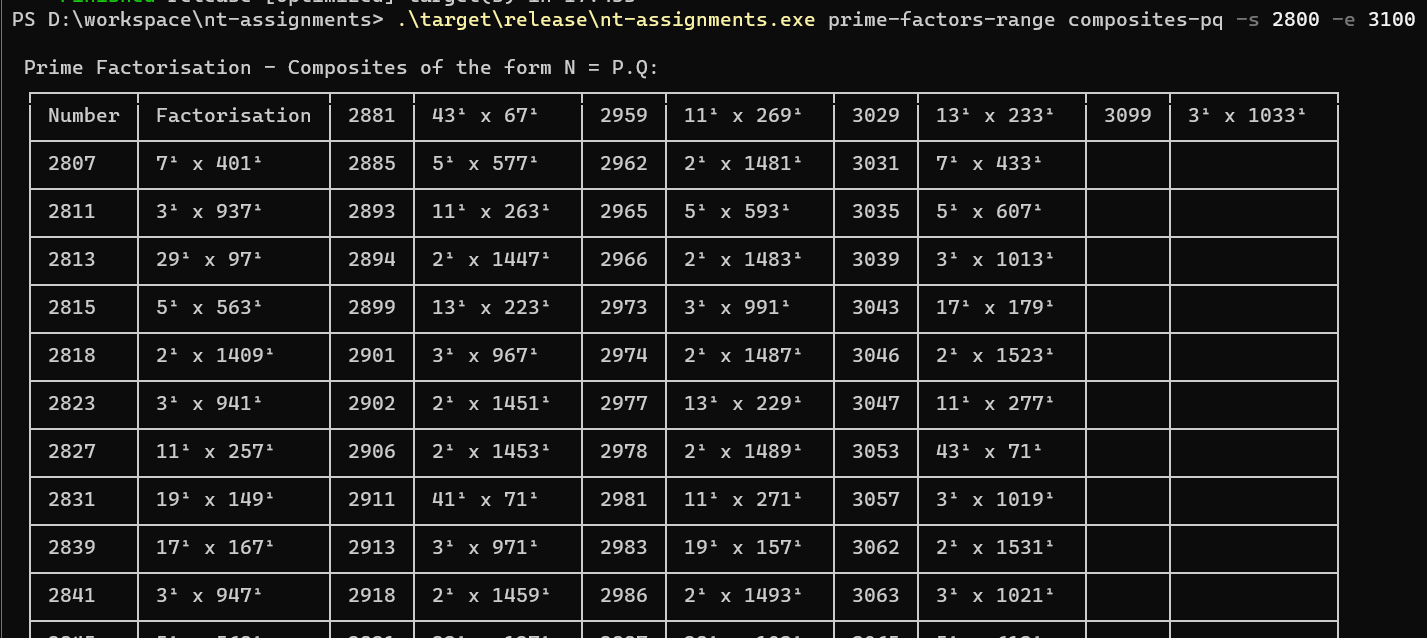
\includegraphics[scale=.45]{n_is_p.q.png}
					\captionof{figure}{Sample output on a Windows terminal}
				\end{center}
			\end{minipage}
			
			\bigbreak
			The below command execution prints numbers of the form $n = p.q$ in a table:
			\begin{lstlisting}[style=DOS, caption=Print numbers of the form n = p.q]
				
			.\target\release\nt-assignments.exe prime-factors-range composites-pq -s 2800 -e 3100
			\end{lstlisting}

		\end{flushleft}
		
		\begin{enumerate}[(c)]
			\item Choose any three element of the set B and then randomly select 4 values of a for each element. Apply the gcd test for each of the 12 cases and report on how accurate it is in determining that a number is composite.  
		\end{enumerate}
		\begin{flushleft}
			\textbf{\textit{Answer:}} The below image shows the output of one execution of the gcd test on three composite numbers selected random in the inclusive range of $2800$ to $3100$.
			
			\begin{minipage}{\linewidth}
				\begin{center}
					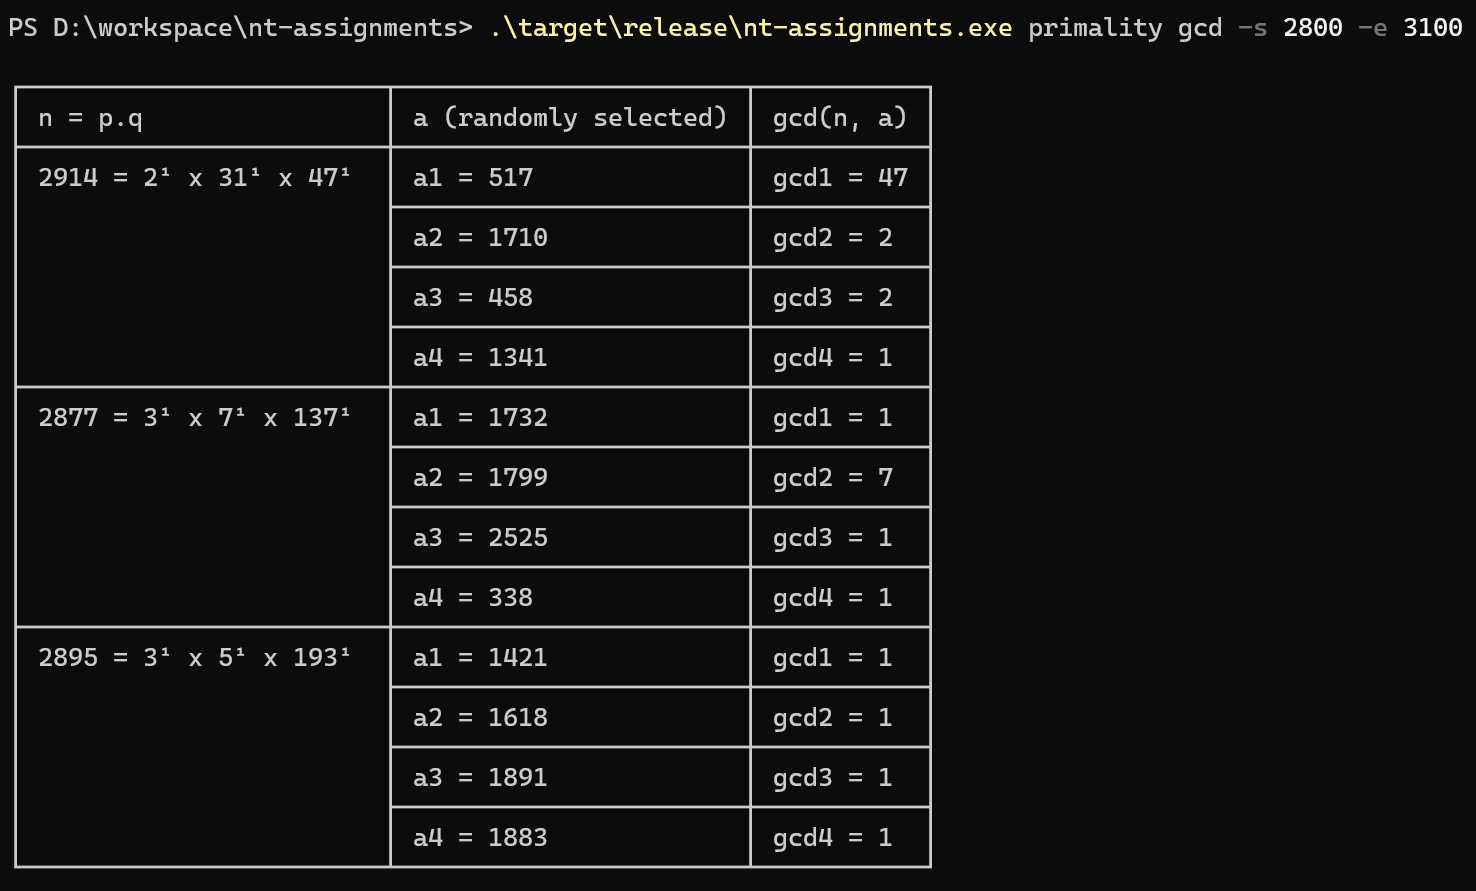
\includegraphics[scale=.45]{gcd_test_3.png}
					\captionof{figure}{Primality Check using GCD Test}
				\end{center}
			\end{minipage}
			\bigbreak
			At the first glance we could see that the composite number $n = 2895$ which has a prime factorisation of $3^1 \times 5^1 \times 193^1$ do not have any Fermat Witnesses to prove that it's a composite number. All the randomly selected $a = \{1421, 1618, 1891, 1883\}$ values yielded  $gcd = 1$ which makes all these $a$ values Fermat Liars. \bigbreak
			The accuracy of GCD Test for primality depends on the selection of the $a$ values. Of course it's not practical to test with all the numbers less than $n$ to find if $n$ is composite. It will turn into the sieving process if we do that. Also, there are cases where some numbers (Carmichael Numbers) do not yield any Fermat Witnesses. The Euler Totient Function $\phi(n)$ gives the total number of relatively prime numbers less than $n$. Which means for a composite number $n$, $n - \phi(n)$ values will attest $n$ is composite. $n - \phi(n)$ becomes smaller when $\phi(n)$ is large. For composite numbers of the form $n = p.q$, that's numbers with fewer prime factors have higher values of $\phi(n)$. \bigskip
			       
			Let's consider the number $n = 2881$
			\begin{align}
				& 2881 = 43^1 \times 67^1 &&\text{(prime factorisation)}\nonumber\\
				& \phi(2881) = 42 \times 66 = 2772 \nonumber\\
				& n - \phi(n) = 109 \approx 4\% \nonumber
			\end{align}
		Only $4\%$ of the numbers are Fermat Witnesses in this case which is much much smaller to form an definite opinion on whether such a number is prime or not when we choose the bases randomly.
		
		\bigbreak
		The below command execution prints output of GCD Test in a table:
		\begin{lstlisting}[style=DOS, caption=GCD Test Execution]
					
		.\target\release\nt-assignments.exe primality gcd -s 2800 -e 3100
		\end{lstlisting}
		
		\bigbreak
		GCD Test Code snippet:
		\begin{lstlisting}[
			language=Rust, 
			basicstyle=\tiny, 
			caption=Code - Primality using GCD Test"  
			]
			
		/// Returns a Vec of randomly selected `a` value and `gcd`
		///
		/// # Arguments
		/// * n - BigInt - Number for which we are checking primality
		/// * num_trials - u8 - How many trials we do
		///
		/// # Examples
		/// ```
		/// use crate::primality::gcd_test
		/// let result: Vec<(BigInt, BigInt)> = gcd_test(&BigInt::from(2881u64), 4);
		/// ```
		///
		pub fn gcd_test(n: &BigInt, num_trials: u8) -> Vec<(BigInt, BigInt)> {
			let mut r = Vec::<BigInt>::new();
			for _ in 0..num_trials {
				r.push(generate_random_int_in_range(&BigInt::from(2u8), &(n - 1)));
			}
			
			let mut result = Vec::<(BigInt, BigInt)>::new();
			for a in r.iter() {
				result.push((a.clone(), n.gcd_euclid(&a)));
			}
			
			result
		}
		
		pub trait Gcd {
			///
			/// # Examples
			///
			/// ```
			/// use utils::Gcd;
			///
			/// assert_eq!(BigInt::from(44u64), BigInt::from(2024u64).gcd_euclid(&BigInt::from(748u64)));
			/// ```
			
			/// Determine [greatest common divisor](https://en.wikipedia.org/wiki/Greatest_common_divisor)
			/// using the [Euclidean algorithm](https://en.wikipedia.org/wiki/Euclidean_algorithm).
			fn gcd_euclid(&self, other: &Self) -> Self;
		}
		
		impl Gcd for BigInt {
			///
			/// GCD Calculator - The Euclidean Algorithm
			/// Input: A pair of integers a and b, not both equal to zero
			/// Output: gcd(a, b)
			///
			fn gcd_euclid(&self, other: &BigInt) -> BigInt {
				let zero = BigInt::from(0u64);
				let mut a = self.clone();
				let mut b = other.clone();
				let mut gcd: BigInt = zero.clone();
				if b > a {
					gcd = b.gcd_euclid(&a);
				} else {
					let mut r: BigInt = &a % &b;
					while &r > &zero {
						// let q = &a / &b;
						r = &a % &b;
						
						if &r != &zero {
							a = b;
							b = r.clone();
						}
					}
					
					gcd = b;
				}
				
				gcd
			}
		}
		\end{lstlisting}
		
		\end{flushleft}
		\bigskip
	
	\begin{enumerate}[2.]
		\item Find all Carmichael Numbers in your range (Lower Range = 2800, Upper Range = 3100) using:

	
	\begin{flushleft}
		\medskip
		\begin{enumerate}[(a)]
			\item A direct method employing the Fermat Test that shows that a composite number n has no Fermat Witnesses. \\
			\medskip
			\textbf{\textit{Answer:}} The below code snippet shows how FLT is employed in finding a Carmichael number:
		
			\begin{lstlisting}[
			mathescape=true,
			language=Rust, 
			basicstyle=\tiny,
			caption=Code - Search Carmichael Numbers in the range"
			label=carmichael-flt  
			]
			
			/// Returns a list of Carmichael Numbers (Absolute Pseudoprimes) in a range using FLT or Korselt's criterion
			///
			/// # Arguments
			/// * start: BigInt
			/// * end: BigInt
			/// * f: a function pointer to either primality::carmichael_nums_korselt or primality::carmichael_nums_flt
			/// # Examples
			/// ```
			/// use crate::presets::list_carmichael_nums;
			/// let carmichael_nums = list_carmichael_nums(&start, &end, carmichael_nums_flt);
			/// ```
			///
			pub fn list_carmichael_nums(start: &BigInt, end: &BigInt, f: fn(&BigInt) -> bool) -> (String, Vec<(BigInt, Vec<(BigInt, usize)>)>) {
				// Get all the composite numbers in the range
				let composites = list_prime_factors_in_range(start, end, NumCategory::Composites).1;
				
				// Searching for Carmichael numbers in parallel
				let carmichael_nums = composites
				.par_iter()
				.filter(|x| f(&x.0) == true)
				.map(|x| x.clone())
				.collect::<Vec<(BigInt, Vec<(BigInt, usize)>)>>();
				
				// Format the data for printing
				let mut table_data: Vec<NumFactorTable> = Vec::new();
				for item in carmichael_nums.iter() {
					let mut form: String = String::new();
					format_prime_factors_print(&item.0, &item.1, &mut form, &mut table_data);
				}
				
				let mut table1 = Table::new(table_data);
				table1.with(STYLE_2);
				
				let output1 = table1.to_string();
				(output1, carmichael_nums)
			}
				
			///
			/// Carmichael Numbers using FLT
			/// n: a composite number
			///
			pub fn carmichael_nums_flt(n: &BigInt) -> bool {
				let n_minus_one = n - 1;
				// Get all the coprime numbers less than `n`
				let coprimes_n = coprime_nums_less_than_n(n);
				
				// Search for Fermat Witnesses. A Fermat Witness will yeild $a^{n-1} \not\equiv 1(mod n)$
				let fermat_witnesses = coprimes_n
				.par_iter()
				.filter(|x| modular_pow(&x, &n_minus_one, n) != BigInt::one())
				.map(|x| x.clone())
				.collect::<Vec<BigInt>>();
				
				// No Fermat Witness means n is a Carmichael Number
				fermat_witnesses.len() == 0
			}
			\end{lstlisting}
			
			When we run the above code, we get $2821 = 7^1 \times 13^1 \times 31^1$ as the Carmichael Number between $2800$ and $3100$ inclusive. A sample execution is given below:
			\bigbreak
			\begin{minipage}{\linewidth}
			\begin{center}
				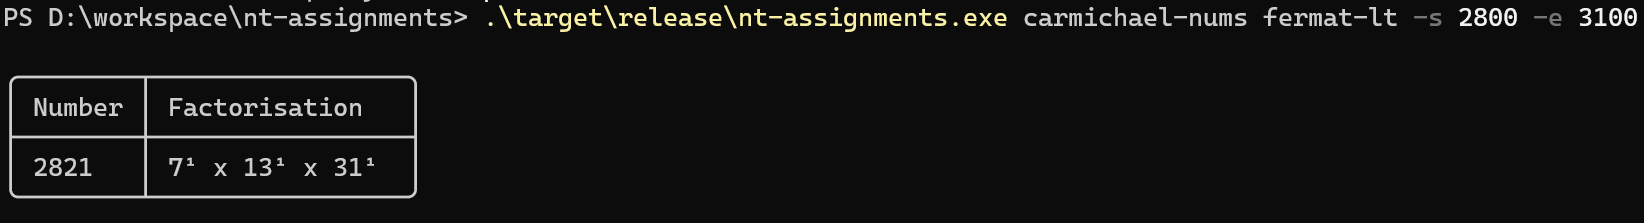
\includegraphics[scale=.45]{carmichael_flt.png}
				\captionof{figure}{Carmichael Number using FLT- Example result}
			\end{center}
			\end{minipage}
			\bigbreak
			
			The below command execution prints Carmichael Numbers in the range using FLT:
			\begin{lstlisting}[style=DOS, caption=Carmichael Numbers using FLT]
				
			.\target\release\nt-assignments.exe carmichael-nums fermat-lt -s 2800 -e 3100
			\end{lstlisting}

			\bigbreak		
			\item Checking which numbers satisfy Korselt’s Criteria.\\
			\medskip
			\textbf{\textit{Answer:}} Korselt's criteria states:
			
			\begin{enumerate}[1.]
				\item $n$ is squarefree i.e. the prime decomposition of $n$ do not contain any repeated factors;
				\item $p | n \implies (p-1) | (n-1)$;
			\end{enumerate}
			
			
			
			\item $\mathbf{|G| = 128}$. \\
			The prime factorization is given by $128 = 2^7$. It's a p-group and hence the center of the group Z(G) is not trivial. Also Z(G) is a proper normal subgroup of G. By Cauchy's theorem, if $|G| = n$ and if $n = pm$ where p is a prime and $p|m$, then $\exists g \in G$ such that $g^p = e \implies |g| = p$\medskip\\
			
			In  our case, we can write $|G|$ as $128 = 2\times2^6$. So $p = 2$ and $m = 2^6$. This implies that we can generate the entire group using the single element 'g', i.e, 
			
			$G = \langle g | g^{128}=e\rangle$ and this is cyclic. Every cyclic group is abelian and hence Z(G) = G, but the order is not prime and hence \textbf{not simple}
			
			\item $\mathbf{|G| = 129}$. Upon prime factorization, $129 = 3\times43$\\. 
			
			By Lagrange's theorem, the order of a subgroup must divide the order of the group. The factors of 129 are $\{1, 3, 43, 129\}$. For a simple group, the only normal subgroups are the trivial group $\{e\}$ and the improper subgroup G itself. So subgroups of order 1 and 129 are out of question here. We need to verify if subgroups of order 3 and 43 are normal.\medskip\\
			
			Let's verify if we have a Sylow 43-subgroup in G. By Sylow's third theorem, $n_{43} \equiv 1(\textrm{mod}\ 43)$ and $n_{43}|3$.\\
			We have $n_{43} = 1$ satisfies the condition. That means there exists a unique proper normal Sylow 43-subgroup for a group of order 129. So the group is \textbf{not simple.}
			
			\item $\mathbf{|G| = 130}$.\medskip\\
			
			$|G| = 2\times5\times13$. If we consider Sylow 13-subgroup in G, by Sylow's third theorem, $n_{13} \equiv 1(\textrm{mod}\ 13)$ and $n_{13}|10$.\\
			Only $n_{13} = 1$ can satisfies these two conditions. That means there exists a unique proper normal Sylow 13-subgroup for a group of order 130. So the group is \textbf{not simple.}
			
			\item $\mathbf{|G| = 131}$.\\
			131 is a prime number. By Lagrange's theorem, the order of a subgroup must divide the order of the group. The only factors of 131 are 1 and 131 itself and hence there are no proper normal subgroups for a group or order 131. So the group is \textbf{Simple.}
			
			\item $\mathbf{|G| = 132}$.\\
			
			The prime factorization of $|G|$ is given by $|G| = 2^2\times3\times11$. We will consider Sylow 11-subgroups first.\\
			The constraints are $n_{11} \equiv 1(\textrm{mod}\ 11)$ and $n_{11}|12$ and $n_{11} = \{1, 12\}$ satisfies these constraints. If $n_{11} = 1$, then the group has a proper normal Sylow 11-subgroup and hence G is not simple. If $n_{11} = 12$, there are 12 subgroups with 10 elements of order 11 in each (the identity element is shared). So The total number of elements of order 11 in G is 120.
			
			Now if we consider Sylow 3-subgroups, the constraints are $n_3 \equiv 1(\textrm{mod}\ 3)$ and $n_3|44$. $n_3 = \{1, 4, 22\}$ satisfies these constraints. Now if we consider $n_3 = 1$, then there exists a proper normal Sylow 3-subgroup and hence G is not simple. If we consider $n_3 = 4$, there exist 4 Sylow 3-subgroups. Hence the total number of elements in the group now is $120 + 4\times2 = 128$. Only 4 elements remaining and a Sylow 2-subgroup of order 4 will fill that. Then the Sylow 2-subgroup is a unique proper normal subgroup hence G is not simple. If we consider $n_3 = 22$, then the total number of elements becomes $120 + 22\times2 = 164$ which is greater than 132 and hence $n_3 = 22$ is not possible.
			
			We will now consider the Sylow 2-Subgroups. The constraints are $n_2 \equiv 1(\textrm{mod}\ 2)$ and $n_2|33$. $n_2 = \{1, 3, 11, 33\}$ satisfies these constraints. If $n_2 = 1$, then there exists a proper normal Sylow 2-subgroup of order 4 and hence the group G is not simple. $n_2 = \{3, 11, 33\}$ will not tally to 132 and hence those values are not possible. So a group of order $|G| = 132$ is not a simple group
		\end{enumerate}
	\end{flushleft}
\end{enumerate}
	\begin{enumerate}[4.]
		\item Let G be a group and suppose H\textsubscript{1} and H\textsubscript{2} are subgroups of G such that there exists $g \in G$ such that $H_1 = H_2 = \{h^g : h \in H\}$
		\begin{enumerate}[(a)]
			\item Show that $H_1 \cong H_2 $.
		\end{enumerate}
		\begin{flushleft}
			\textbf{\textit{Answer:}}
			Given $H_1, H_2 \le G$ 
			
			Let $\sigma$ be the isomorphic mapping from $H_1$ to $H_2$. Then $\sigma$ is given by:
			$\sigma_g: H_1 \to H_2$ and is defined as $\sigma_g: h \mapsto ghg^{-1}$, $\forall h \in H_1$. Let $h_1, h_2 \in H_1$. Then for an isomorphism, the following constraint must be satisfied along with the mapping $\sigma$ being bijective.
			
			$\sigma(h_1h_2) = \sigma(h_1)\sigma(h_2)$
			
			LHS: $\sigma(h_1h_2) = g(h_1h_2)g^{-1}$
			RHS: $\sigma(h_1)\sigma(h_2) = gh_1g^{-1}gh_2g^{-1} = gh_1eh_2g^{-1} = gh_1h_2g^{-1}$
			
			Hence $LHS = RHS$ and $\sigma$ is a homomorphism.
			
			Proof for Bijection: We can prove it by showing $\sigma_g$ has two sided inverse, that's if $\sigma_g^{-1} = h: \mapsto g^{-1}hg$ then we need to prove $\sigma_g^{-1}(\sigma_g(h)) = h$, $\forall h \in H1$ and $\sigma_g(\sigma_g^{-1}(h)) = h$, $\forall h \in H1$
			
			1. $\sigma_g^{-1}(\sigma_g(h)) = \sigma_g^{-1}(ghg^{-1}) = g^{-1}(ghg^{-1})g = h$\\
			2. $\sigma_g(\sigma_g^{-1}(h)) = \sigma_g(g^{-1}hg) = g(g^{-1}hg)g^{-1} = h$
			
			Hence the mapping is bijective. $\therefore H_1 \cong H_2 $
		\end{flushleft}
		\begin{enumerate}[(b)]
			\item Now suppose that G is finite and that $P, P^{\prime} \in Syl_p(G)$. Explain why $P$ and $P^{\prime}$ are isomorphic.
		\end{enumerate}
		\begin{flushleft}
			\textbf{\textit{Answer:}}
			If we have $P, P^{\prime} \in Syl_p(G)$ then they are conjugates in G by Sylow's second theorem. i.e, $\exists g \in G$ such that  $P^{\prime} = gPg^{-1}$. Conjugate groups are always isomorphic.
		\end{flushleft} 
	\end{enumerate}
\end{enumerate}
	
	\begin{thebibliography}{unsrt}
		
		\bibitem{Modular_Mathematics}
		C R Jordan \& D A Jordan \emph{MODULAR MATHEMATICS Groups }.
		
		\bibitem{gt_solutions}
		Dr. Ben Fairbairn \emph{GROUP THEORY Solutions to Exercises}.
		
		\bibitem{online_ref_1}
		\emph{https://yutsumura.com/sylows-theorem-summary/}
		
	\end{thebibliography}
	
\end{document}